\chapter{航天器姿态运动学}
\thispagestyle{empty}

\section{航天器常用坐标系}
\subsection{基本概念}
\vspace*{-0.5em}

\defination[天体坐标系基本概念]
{
	\dy[天球]{TQ}\quad 指一个以地球质心$M$为中心,半径$r$为任意长的一个假想的球体 。其目的是将天体沿观测者视线投影到球面上,以便于研究天体及其相互关系。\\
	\hspace*{2.2em}\dy[黄道平面]{HDPM}\quad 由于地球绕太阳公公转而产生的,即地球公转轨道在天球上的反映称为黄道。它和赤道面相交于春分点和秋分点。\\
	\hspace*{2.2em}\dy[春分点]{CFD}\quad 指太阳从难向北在黄赤道上的交点。
}

\begin{figure}[!htb]
	\begin{minipage}{0.45\linewidth}
		\centering
		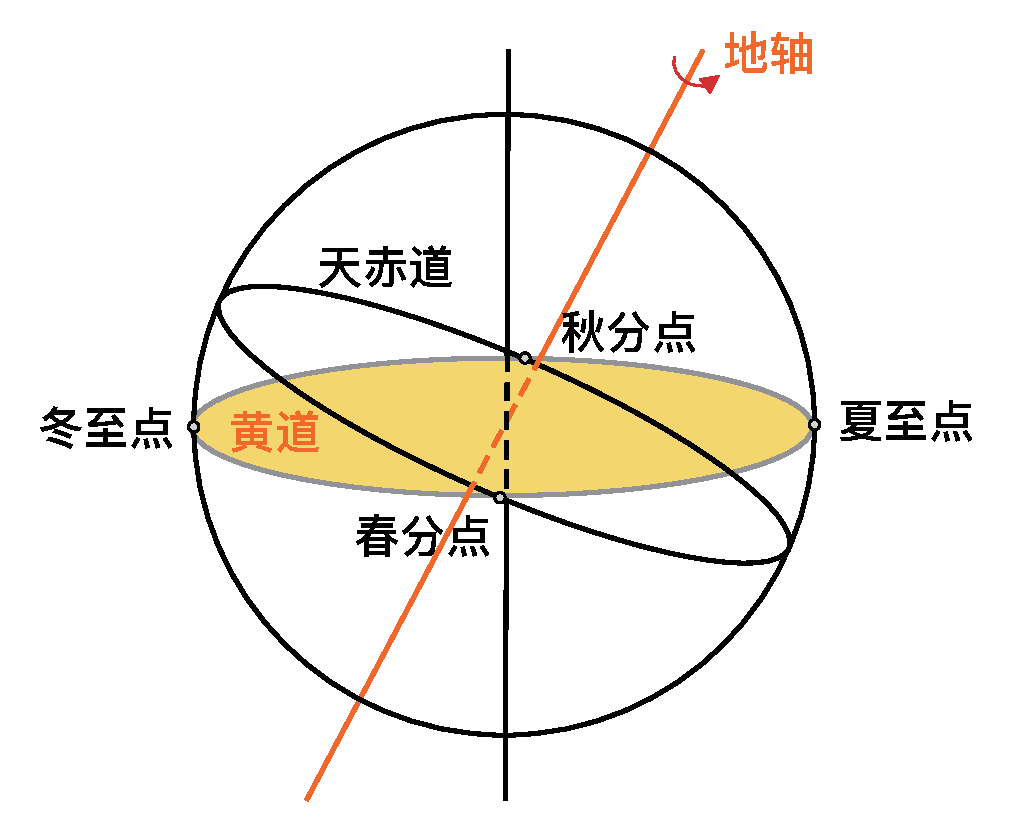
\includegraphics[width=\linewidth]{pic/基本概念}
		\caption{天球坐标系的基本概念}
		\label{基本概念}
	\end{minipage}
	\begin{minipage}{0.55\linewidth}
		\centering
		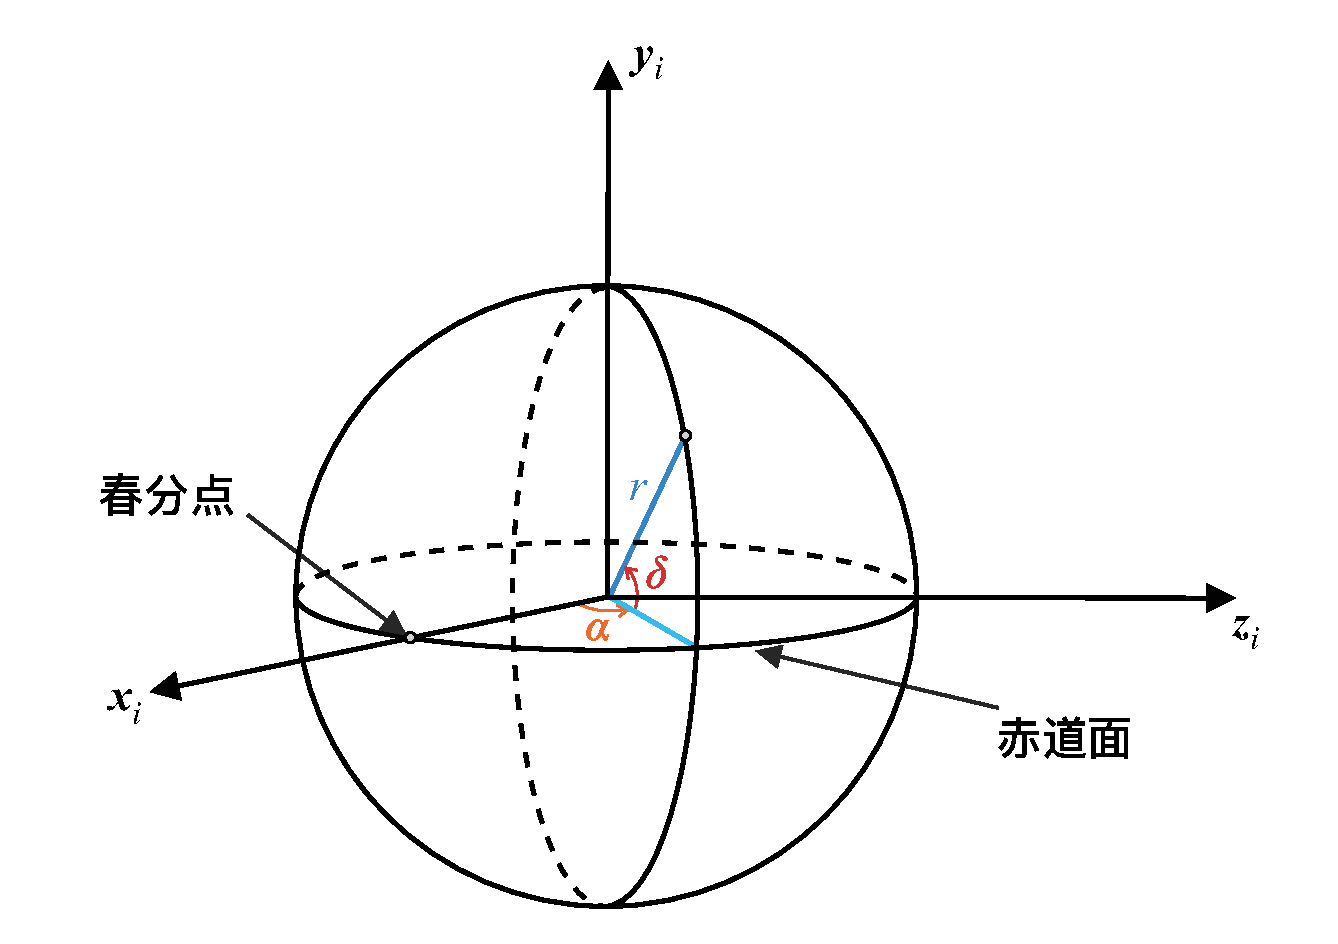
\includegraphics[width=\linewidth]{pic/地惯}
		\vspace*{-2.9em}
		\caption{地心赤道惯性坐标系}
		\label{基本概念}
	\end{minipage}
\end{figure}

\subsection{地心赤道惯性坐标系}
\vspace*{-0.5em}

\defination[地心赤道惯性坐标系]
{
	如图所示,\dy[地心第一赤道坐标系]{DXDYCDZBX},简称为\dy[惯性坐标系]{GXZBX}。$X$轴在地球赤道平面内,指向赤道平面与黄道平面的相交线交点(春分点)。$Z$轴垂直于赤道平面,与地球自转角速度矢量方向一致。J2000的地心平赤道、平春分点的地心赤道坐标系。
}



















